\chapter{Introducción}
\drop{D}{esde} la introducción del ordenador personal en la década de los años 80, los esfuerzos por naturalizar la experiencia de la interacción ha estado limitada por el factor de adaptación de una persona a los distintos entornos informáticos. A día de hoy, todavía conservamos el mismo esquema de utilización de un ordenador de sobremesa de principios de los 80, con computadores que tienen prácticamente la misma configuración de monitor, teclado y ratón. Realmente no hay nada de natural en este tipo de experiencia de usuario, y en todo caso es lo más alejado de ser una función humana. Para apoyar aún más lo lejos que nos hemos desviado de esta naturaleza, el estudio de la ergonomía surgió como una manera de minimizar en nuestros cuerpos el riesgo de una lesión, ya que tratamos de adaptarlos a este entorno no natural.

Afortunadamente vivimos en una época en la que estamos rompiendo con los paradigmas tradicionales establecidos. La introducción de nuevas formas de relacionarnos con los ordenadores esta haciendo que vean la luz dispositivos portátiles, superficies multitáctiles, proyecciones interactivas,... donde estamos dejando las limitaciones de los entornos virtuales y metáforas obsoletas. Ya es hora de que volvamos a nuestro mundo natural.

\section{Un poco de historia}
Los computadores hasta los años 70, no eran mucho más que grandes calculadoras utilizadas para automatizar cálculos complejos en instituciones militares y para investigación de alto nivel en unas pocas universidades. Las primeras interfaces consistían en introducir una serie de tarjetas perforadas que contenían el programa codificado y más tarde revisar en un impresora el resultado de la ejecución.

Posteriormente se desarrollaron las interfaces de línea de comandos (CLI), así el usuario ya no tuvo que perforar tarjetas ni tenía que esperar. Los programadores y usuarios disponían de acceso a un terminal, y lo usaban para interactuar directamente con el ordenador en algo parecido a lo que podemos denominar ``tiempo real''. El usuario podía introducir una orden, y obtener una salida textual de vuelta más o menos inmediata.

Fue a principios de los años 80, cuando la informática dio un gran salto mediante la interfaz gráfica de usuario (GUI), que era una forma más natural y convincente para interactuar con un ordenador. Esto hizo que la informática fuese más accesible para la gente, dándole la capacidad de comunicarse con el ordenador a base de metáforas de escritorio, ventanas y punteros de ratón.

Pero en los 30 años desde el lanzamiento del primer ordenador en ofrecer una interfaz gráfica de usuario en una máquina de bajo coste, la experiencia física de la interacción no ha sufrido muchos cambios en lo que se refiere a ordenadores personales. En este tiempo se inventó la Web, progresó desde su primera iteración hasta el actual HTML 5, desarrollamos multitud de revolucionarias plataformas web para conectar y relacionarnos por todo el mundo, pero mantenemos nuestra rígida adhesión al legado del monitor, ratón y teclado a principios de 2010 como lo fue en la década de los 80. 

\section{Volviendo a lo natural}
No es hasta finales de los años 2000, cuando podemos decir que empieza la «era post-PC». La generalización de los dispositivos multi-touch y la informática móvil marca uno de los mayores hitos en las interfaces persona-computador. Los dispositivos móviles se diseñan para ser ligeros, portátiles y encajar con nuestro estilo de vida personal. De repente, estamos en medio de una de las más importantes revoluciones tecnológicas, cuando nuestros dispositivos informáticos comienzan a adaptarse a nuestras funciones naturales humanas.

El primer paso en este ámbito ha sido la amplia adopción de la tecnología móvil inteligente en las funciones cotidianas, como por ejemplo, el control de una agenda con los planes del día o saber a dónde ir, independientemente del sentido de orientación que tengamos. El conocimiento aparece en el momento que sacamos el smartphone en busca de las respuestas.

Apenas estamos comenzando a descubrir las posibilidades de un mundo en el que los dispositivos se adaptan a nuestras conductas y la tecnología apoya y amplifica nuestras funciones naturales. Estaremos en el camino de lo que podemos llamar «computación humana», cuando el hardware desaparezca y nos pase desapercibido que realmente estamos interaccionado con un ordenador. Esto ocurre cuando la tecnología se integra discretamente en objetos cotidianos o en funciones naturales. La tecnología será la que se adapte a nosotros, en lugar de ser nosotros quienes se adapten a la computación y la máquina aprenda a reconocer e interpretar los patrones humanos para producir una salida basada en un contexto familiar.

Un ejemplo de una tecnología no relacionada con la computación que ha madurado con el tiempo, es la optometría. Basta con pensar en las lentes de contacto. Se coloca una capa fina directamente en nuestra córnea, alterando así los rayos de luz que convergen perfectamente en nuestra retina. Al instante, sin apenas esfuerzo, tenemos una visión perfecta. Una vez colocadas tendemos a olvidar que las llevamos puestas y esto se debe a su perfecta integración en nuestro estilo de vida cotidiana. 

Para reflexionar sobre el estado actual de la informática en relación a la optometría: imaginemos que dependiésemos de un teclado y un ratón para modificar nuestra vista cada vez que necesitásemos enfocar.

\section{Interfaces naturales basadas en visión artificial}
\emph{Interfaz natural de usuario} es un término genérico para una variedad de tecnologías que permiten a los usuarios interactuar con los ordenadores en términos humanos. Algunas de estas tecnologías son las basadas en visión por computador y que son capaces desde interpretar expresiones naturales como gestos hasta proporcionar información contextual que se proyecta dentro del campo de visión del usuario, como pretenden las Google Glass. 

Las interfaces de usuario basadas en visión por computador llevan varios años desarrollándose y comercializándose con éxito dentro de la industria del videojuego. Mediante un dispositivo externo permite a los usuarios controlar e interactuar con la consola sin necesidad de tener contacto físico con un controlador de videojuegos tradicional, reconociendo gestos, comandos de voz, objetos e imágenes.

\subsection{EyeToy}
El EyeToy es un cámara que fue lanzada en octubre de 2003 para la PlayStation 2. Este dispositivo utiliza visión por computador y reconocimiento de gestos para procesar las imágenes adquiridas por la cámara y permite a los jugadores interactuar con los juegos.

La estética de los juegos que soportaban este sistema consistían en la introducción del jugador en la pantalla mediante realidad mixta y mediante la realización de determinados gestos, sea el personaje en el que se basa la historia del juego. 

\begin{figure}[b] % indico que voy a poner una figura y [h] indica que la posición relativa, tambien puedo usar t = top entre otros.
\hfill
\begin{minipage}[t]{.45\textwidth}
\begin{center}
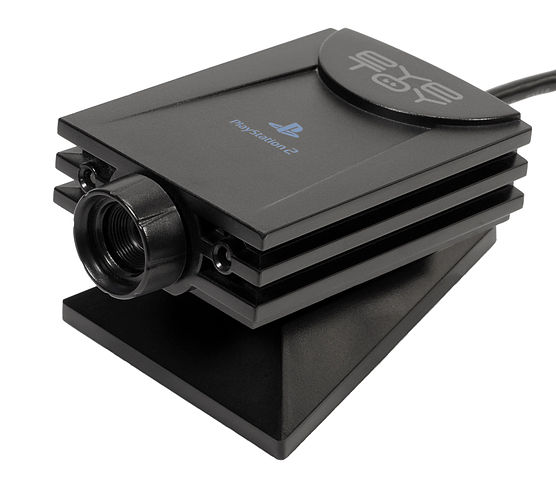
\epsfig{file=eyetoy.jpg, scale=0.3} % primera imagen colocada a la izquierda
\caption{EyeToy para PlayStation 2}
\label{eyeToy}
\end{center}
\end{minipage}
\hfill
\begin{minipage}[t]{.45\textwidth}
\begin{center}
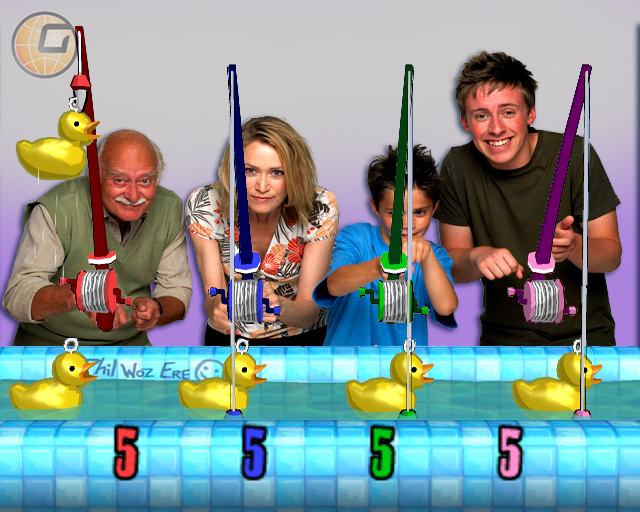
\epsfig{file=eyetoy-game.jpg, scale=0.3} % segunda imagen colocada a la derecha 
\caption{EyeToy Play 3 con los jugadores inmersos en el juego.}
\label{eyetoy-game}
\end{center}
\end{minipage}
\hfill
\end{figure}

Este tipo de interación supuso una revolución en la forma de interactuar con los videojuegos, vendiendo más de 10 millones de unidades por todo el mundo, y ha sido precursor de otros dispositivos como Kinect.

\subsection{Kinect}
Kinect es un sensor que se vendió previamente como un periférico opcional, por 150 euros, para la videoconsola Xbox 360 y posteriormente para Xbox One y Windows, debido al gran éxito obtenido. Según datos de Microsoft, a principios de 2013 se habían comercializado más de 24 millones de Kinect. 

\begin{figure}
  \centering
  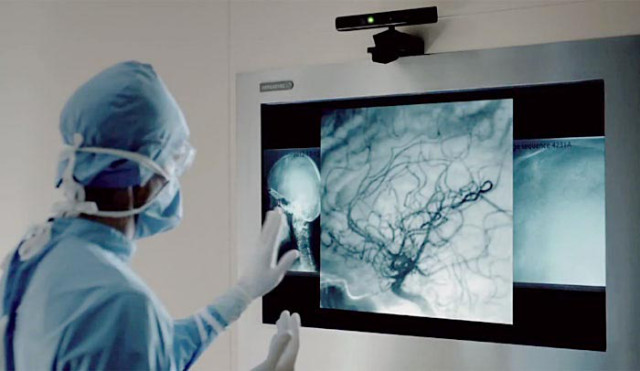
\includegraphics[width=1.0\textwidth]{kinect-health.jpg}
  \caption{Utilización de Kinect para la visualización de radiografías durante una cirugía}
  \label{fig:kinect-health}
\end{figure}

%\begin{figure}[h] 
%  \centering
%  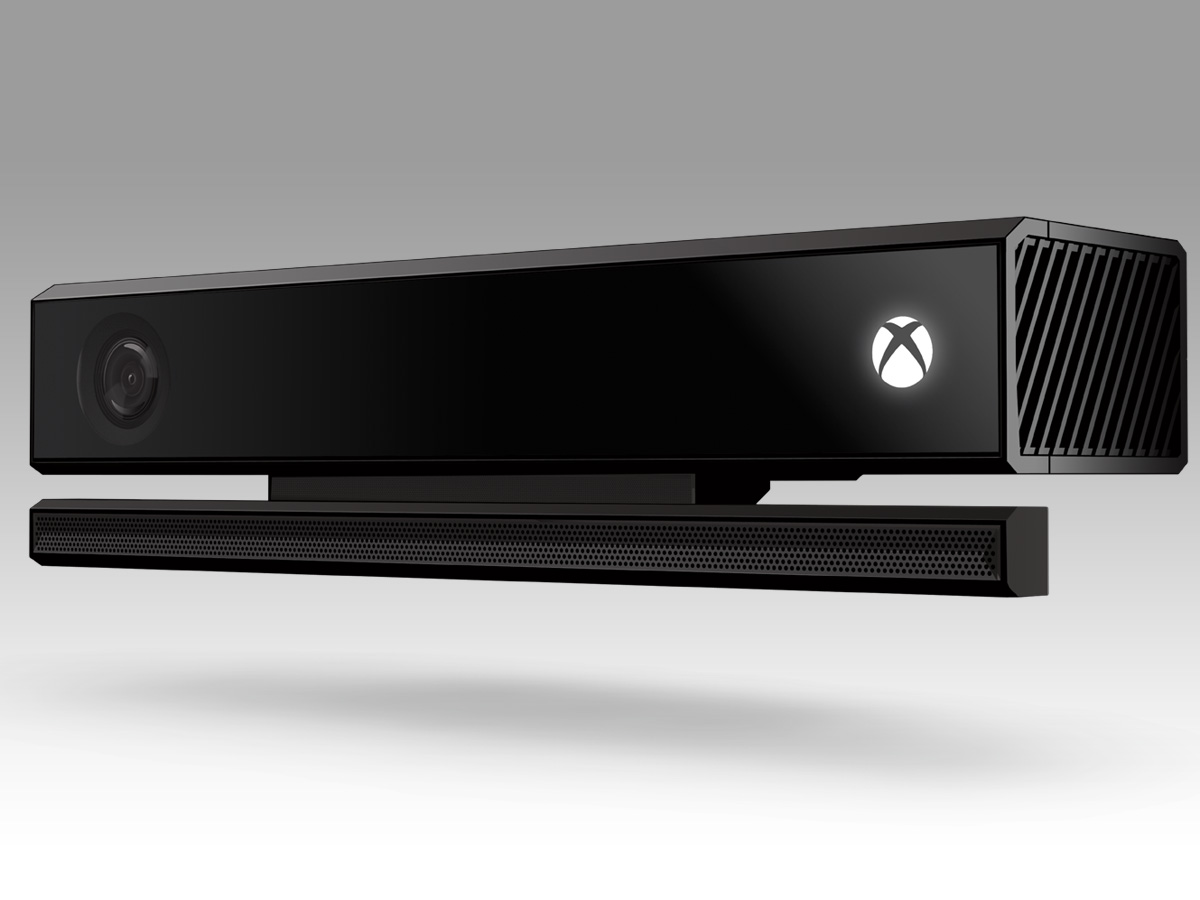
\includegraphics[width=0.5\textwidth]{kinect.jpg}
%  \caption{Kinect para Microsoft Xbox One}
%  \label{fig:kinect}
%\end{figure}


El dispositivo cuenta con una cámara RGB, un sensor de profundidad y un vector de micrófonos que le permite distinguir extremidades y los movimientos realizados con ellas, expresiones faciales, gestos con las manos y los dedos, incluso el pulso del usuario, y utilizarlos para controlar e interactuar con la consola. Gracias a los micrófonos es capaz de reconocer la dirección del origen del sonido y proporcionar cancelación de ruido.

Estas interesantes características motivaron a la comunidad de usuarios para obtener una solución de código abierto y utilizar el dispositivo en cualquier ordenador y no únicamente en la consola de videojuegos. Varios días después de su lanzamiento, se publicó el primer controlador para ordenador obtenido mediante ingeniería inversa. Esto dio paso a la creación de varias APIs libres que han permitido el uso del Kinect de forma no oficial más allá de lo que en un principio se hubiese esperado, impulsando el interés en explorar nuevas modalidades de interacción. Finalmente Microsoft liberó un SDK para desarrollo de aplicaciones con el dispositivo en Windows.  

\section{Realidad Aumentada}
La realidad aumentada se podría considerar como la aplicación de distintas técnicas de visión por computador, mediante la cual la percepción del mundo real se complementa con información adicional generada por ordenador en tiempo real. Esta información adicional puede ser desde etiquetas virtuales, representaciones de modelos tridimensionales, o incluso cambios de iluminación. 

\begin{figure} 
  \centering
  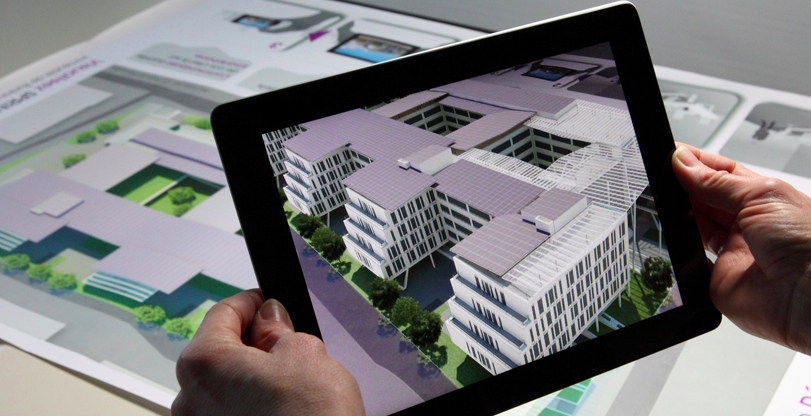
\includegraphics[width=1.0\textwidth]{augmented_example.jpg}
  \caption{Previsualizacion 3D mediante realidad aumentada en arquitectura}
  \label{fig:ar_example}
\end{figure} 

%El principal problema que deben tratar los sistemas de realidad aumentada se considera \textbf{registro}, que consiste en calcular la posición relativa de la cámara respecto a la escena para colocar correctamente las imágenes sintéticas dentro de la imagen real. Los objetos del mundo real y virtual deben estar perfectamente alineados o la sensación de integración se verá seriamente afectada.

La realidad aumentada se puede aplicar a prácticamente todos los campos. En el sector industrial, para la reparación y mantenimiento de máquinas e instalaciones complejas, visualización de datos o simulación.  En aplicaciones médicas, mostrarían la situación de órganos no visibles durante una cirugía. También se han realizado aplicaciones para diseño de interiores, presentaciones de productos, educación, publicidad, turismo, arte y ocio. 

%Las aplicaciones de Realidad Aumentada deben cumplir las siguientes características definidas por Ronald T. Azuma \cite{Azuma}:

%\begin{description}
%\item[Combinar el mundo real con el virtual.] El resultado final debe mostrar la información sintética sobre las imágenes percibidas del mundo real.
%\item[Debe ser interactivo en tiempo real.] La integración debe ser realizada \emph{en el momento}, por lo que el cálculo necesario debe realizarse en el menor tiempo posible.
%\item[La alineación de los elementos virtuales debe realizarse en 3D.] Los objetos sintéticos deben de estar correctamente alineados en el espacio tridimensional,  o la sensación de integración se verá seriamente afectada.
%\end{description}

Hoy en día, la mayoría de las aplicaciones de realidad aumentada se centran en la movilidad. De este modo, las pantallas de dispositivos portátiles y los smartphones se han convertido en la opción dominantes para la visualización. Sin embargo, el aumento de las prestaciones y la reducción de los costes hacen que los proyectores se hayan popularizado y establecido como herramientas habituales para la visualización. La capacidad de generar imágenes mucho mayores que el propio dispositivo prácticamente en cualquier lugar es una característica interesante para muchas aplicaciones que no pueden ser mostradas en pantallas convencionales. 

Existen actualmente muchas líneas de investigación sobre este tema, en las que se pretende aplicar este potencial mediante la utilización de los proyectores de una manera poco convencional y desarrollar nuevas e innovadoras pantallas de información que van más allá de presentaciones en las típicas pantalla planas.
 
Los enfoques basados en proyectores combinan las ventajas de la realidad virtual y la realidad aumentada proporcionando sensaciones inmersivas que se pueden realizar sobre entornos cotidianos, sin la necesidad de pantallas de proyección especiales y configuraciones de pantalla dedicadas. Para muchas aplicaciones, esto requiere la perdida de la movilidad, pero no necesariamente de la portabilidad. Otras aplicaciones, sin embargo, no requieren movilidad y más bien se benefician de las propiedades aumentadas que proporciona la proyección. Los ejemplos van desde entretenimiento educativo en los museos, con proyecciones sobre paredes o sobre las propias obras de arte, hasta proyecciones en fachadas de edificios históricos para conseguir efectos de movimiento ó 3D, dando lugar a un espectáculo artístico conocido como \emph{projection mapping.}

\begin{figure} 
  \centering
  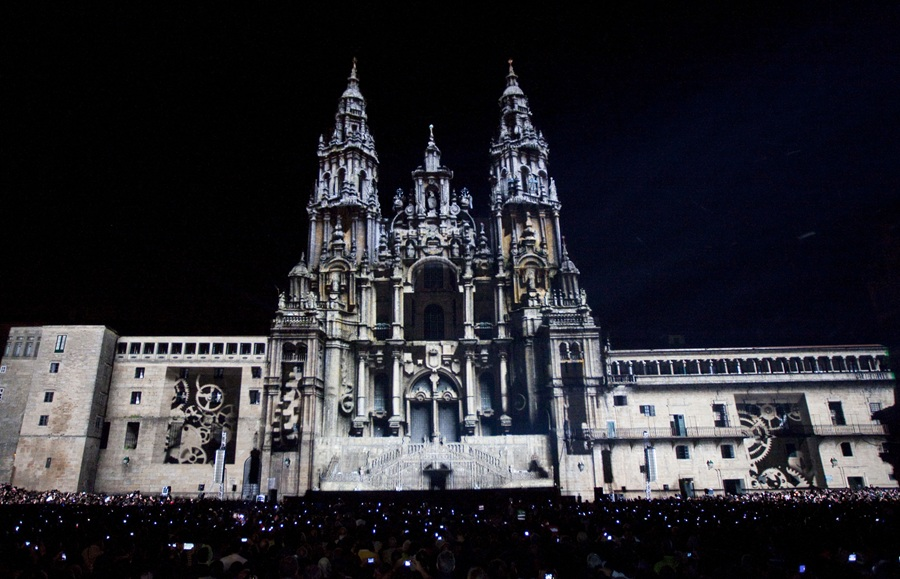
\includegraphics[width=1.0\textwidth]{mapping.jpg}
  \caption{\textit{Projection mapping} realizado sobre la catedral de Santiago en 2011}
  \label{fig:mapping}
\end{figure}

\section{Motivación}

El presente proyecto se enmarca dentro de la Cátedra Indra-UCLM, en el proyecto “ARgos: Sistema de Ayuda a la Gestión Documental basado en Visión por Computador y Realidad Aumentada” que tiene como objetivo la construcción de un sistema de ayuda a la gestión de documentos, basado principalmente en visión por computador y síntesis visual y auditiva en el espacio físico, empleando técnicas de realidad aumentada. 

Todos los países de la Unión Europea aceptan las recomendaciones generales de la Organización Mundial de la Salud así como las directrices y programas de las Naciones Unidas relativas a las personas con necesidades especiales y que proponen expresamente «su participación plena en la vida social, con oportunidades iguales a las del resto». El proyecto esta pensado para facilitar la integración laboral, sean cuales sean las necesidades especiales de las personas que tenga que gestionar documentación impresa. 
  
\section{Impacto socio-económico}
Bajo el concepto de «discapacidad», se incluyen limitaciones muy diversas que afectan con mayor o menor gravedad las facultades que son habituales para desenvolverse en la vida cotidiana y que no tienen por qué impedir una inserción social y laboral normalizada. A día de hoy, las personas con discapacidad pueden desempeñar las funciones laborales, normalmente, gracias a la ayuda de aparatos o de procesos específicos de adaptación del puesto de trabajo. E incluso, una discapacidad total, no significa que el sujeto no pueda suplir o compensar su limitación mediante el uso de otras facultades. 

Según un estudio \cite{OIT} realizado por la Organización Internacional del Trabajo (OIT) se identifican varios tipos de beneficios socio-económicos en la inclusión de personas con discapacidad al mundo laboral.

La persona con discapacidad que trabaja, se convierte en un aporte para la economía del hogar, ya sea porque aporta ingresos o porque autofinancia sus necesidades. Esto disminuye la precariedad de recursos a los que se suelen enfrentar. Al mismo tiempo, incrementa su autonomía respecto de terceros, como su propia familia o instituciones de apoyo. Como consecuencia, la familia gana tiempo y ahorra recursos que antes destinaba al cuidado o manutención de esa persona. 

En el estudio se señala que el sólo hecho de incluir a las personas con discapacidad en la empresa, genera un efecto motivador en otros trabajadores, causa sentimientos de orgullo respecto de la empresa y hace sentir que ésta es un mejor lugar para trabajar. Las empresas inclusivas aumentan su capital simbólico y reputación, aumentando el nivel de aprobación que reciben desde el interior de la propia empresa y desde el entorno. Finalmente, algunas empresas (con más experiencia inclusiva) señalan que la participación de personas con discapacidad en su equipo se traduce en beneficios relacionados con la productividad, ya que estos trabajadores serían especialmente hábiles para la ejecución de ciertas tareas y especialmente comprometidos con la empresa tras acceder a un puesto de trabajo. 

Los beneficios sociales identificados radican en el plano de la cultura, pues se indica que la inclusión cambia la base emocional de la exclusión (desinformación, miedo, prejuicio, mito). Aumenta la valoración social de la diversidad  y cambia positivamente el modo colectivo de convivir e influye en la disminución del conflicto intercultural entre personas con y sin necesidades especiales.
 
\section{Estructura del documento}

  Este documento se ha estructurado según las indicaciones de la normativa de trabajos de fin de grado de la Escuela Superior de Informática de la Universidad de Castilla-La Mancha, y contará con los siguientes capítulos:


  \begin{definitionlist}
  \item[Capítulo \ref{chap:objetivos}: \nameref{chap:objetivos}] Se realiza una exposición concreta de problema a resolver, describiendo el entorno de trabajo, la situación y qué se pretende obtener a modo de requisitos del sistema.

  \item[Capítulo \ref{chap:antecedentes}: \nameref{chap:antecedentes}] Se resumen los antecedentes teóricos y conceptuales y estudios ya existentes, describiendo hechos clave, estado actual y la evolución de la problemática de la visión por computador en el ámbito científico y disciplinar relacionada con el desarrollo de GrayAR.

  \item[Capítulo \ref{chap:metodo}: \nameref{chap:metodo}] Analiza el diseño metodológico escogido, con el fin de responder cómo se ha llevado a cabo el desarrollo de GrayAR, los métodos que se han seguido y la forma de conseguir los objetivos planeados mediante las sucesivas iteraciones. También se describen los recursos empleados, tanto hardware como software.

  \item[Capítulo \ref{chap:arquitectura}: \nameref{chap:arquitectura}] Describe el diseño e implementación del sistema, detallando los problemas surgidos y las soluciones aportadas. Se estructura acorde a los módulos y submódulos que componen el sistema, dando primero una visión general y funcional del módulo, y pasando posteriormente a los detalles técnicos y de implementación. 

  \item[Capítulo \ref{chap:resultados}: \nameref{chap:resultados}] Detalla los resultados obtenidos mediante el análisis de rendimiento del sistema, costes económicos del proyecto y estadísticas del repositorio. El objetivo de este estudio es obtener parámetros de referencia que permitan evaluar nuestro sistema respecto a otros productos que posean funcionalidades iguales o similares.

  \item[Capítulo \ref{chap:conclusiones}: \nameref{chap:conclusiones}] Muestra un análisis del trabajo realizado y los objetivos conseguidos. Incluye una descripción de posibles líneas de trabajo futuro sobre el proyecto y una valoración personal del trabajo realizado.

  \end{definitionlist}



  % Local Variables:
  % coding: utf-8
  % mode: latex
  % mode: flyspell
  % ispell-local-dictionary: "castellano8"
  % End:
